\uuid{zjvO}
\exo7id{5735}
\titre{exo7 5735}
\auteur{rouget}
\organisation{exo7}
\datecreate{2010-10-16}
\isIndication{false}
\isCorrection{true}
\chapitre{Suite et série de fonctions}
\sousChapitre{Continuité, dérivabilité}
\module{Analyse}
\niveau{L2}
\difficulte{}

\contenu{
\texte{
Pour $n\in\Nn^*$ et $t\in\Rr$, soit $f_n(t) =\frac{\Arctan(nt)}{n^2}$.

  
Etude complète de $f =\sum_{n=1}^{+\infty}f_n$ : domaine de définition, parité, limites, continuité, dérivabilité (vérifier que $f$ n'est pas dérivable en $0$), allure du graphe.
}
\reponse{
\textbf{Domaine de définition.} Soit $t\in\Rr$. Pour chaque $n\in\Nn^*$, $f_n(t)$ existe et de plus $f_n(t)=\frac{\Arctan(nt)}{n^2}\underset{n\rightarrow+\infty}{=}O\left(\frac{1}{n^2}\right)$. Donc la série numérique de terme général $f_n(t)$, $n\geqslant1$, converge absolument et en particulier converge. On a montré que

\begin{center}
\shadowbox{
$f$ est définie sur $\Rr$.
}
\end{center}

\textbf{Parité.} Pour tout réel $t$,

\begin{center}
$f(-t)=\sum_{n=1}^{+\infty}\frac{\Arctan(-nt)}{n^2}=-\sum_{n=1}^{+\infty}\frac{\Arctan(nt)}{n^2}=-f(t)$.
\end{center}

\begin{center}
\shadowbox{
$f$ est impaire.
}
\end{center}

\textbf{Convergence normale.} Pour tout réel $t$ et tout entier naturel non nul $n$, $|f_n(t)|\leqslant\frac{\pi}{2n^2}$ et donc pour tout entier naturel non nul $n$,

\begin{center}
$\underset{t\in\Rr}{\text{sup}}|f_n(t)|\leqslant\frac{\pi}{2n^2}$.
\end{center}

\rule[-4mm]{0mm}{0mm}Comme la série numérique de terme général $\frac{\pi}{2n^2}$, $n\geqslant1$, converge, la série de fonctions de terme général $f_n$ converge normalement et donc uniformément vers $f$ sur $\Rr$.

\textbf{Limite de $f$ en $+\infty$.} Puisque la série de fonctions de terme général $f_n$, $n\geqslant1$, converge uniformément vers $f$ sur $\Rr$ et que chaque fonction $f_n$ a une limite réelle quand $t$ tend vers $+\infty$ à savoir $\ell_n=\frac{\pi}{2n^2}$, le théorème d'interversion des limites permet d'affirmer que $f$ a une limite réelle en $+\infty$ et que

\begin{center}
$\lim_{t \rightarrow +\infty}f(t)=\sum_{n=1}^{+\infty}\ell_n=\frac{\pi}{2}\sum_{n=1}^{+\infty}\frac{1}{n^2}=\frac{\pi^3}{12}$.
\end{center}

\begin{center}
\shadowbox{
$\lim_{t \rightarrow +\infty}f(t)=\frac{\pi^3}{12}$ et $\lim_{t \rightarrow -\infty}f(t)=-\frac{\pi^3}{12}$.
}
\end{center}

\textbf{Continuité.} Puisque chaque fonction $f_n$, $n\in\Nn^*$, est continue sur $\Rr$ et que la série de fonctions de terme général $f_n$ converge uniformément vers $f$ sur $\Rr$, la fonction $f$ est continue sur $\Rr$ en tant que limite uniforme sur $\Rr$ d'une suite de fonctions continues sur $\Rr$.

\begin{center}
\shadowbox{
$f$ est continue sur $\Rr$.
}
\end{center}

\textbf{Dérivation.} Soit $a>0$. Chaque fonction $f_n$, $n\geqslant1$, est de classe $C^1$ sur $[a,+\infty[$ et pour $n\in\Nn^*$ et $t\geqslant a$,

\begin{center}
$f_n'(t)=\frac{n}{n^2(1+n^2t^2)}=\frac{1}{n(1+n^2t^2)}$.
\end{center}

Pour $n\in\Nn^*$, on a alors $\underset{t\in[a,+\infty[}{\text{sup}}|f_n'(t)|=f_n'(a)=\frac{1}{n(1+n^2a^2)}$. Puisque $\frac{1}{n(1+n^2a^2)}\underset{n\rightarrow+\infty}{\sim}\frac{1}{a^2n^3}>0$, la série de terme général $\frac{1}{n(1+n^2a^2)}$ converge et par suite, la série de fonctions de terme général $f_n'$, $n\geqslant1$, converge normalement et donc uniformément sur $[a,+\infty[$.

En résumé,

\textbullet~la série de fonctions de terme général $f_n$, $n\geqslant 1$, converge simplement vers $f$ sur $[a,+\infty[$,

\textbullet~chaque fonction $f_n$ est de classe $C^1$ sur $[a,+\infty[$,

\textbullet~la série de fonctions de terme général $f_n'$ converge uniformément sur $[a,+\infty[$.

D'après un corollaire du théorème de dérivation terme à terme, $f$ est de classe $C^1$ sur $[a,+\infty[$ et sa dérivée s'obtient par dérivation terme à terme. Ceci étant vrai pour tout $a>0$, $f$ est de classe $C^1$ sur $]0,+\infty[$ et puisque $f$ est impaire

\begin{center}
\shadowbox{
$f$ est de classe $C^1$ sur $\Rr^*$ et $\forall t\in\Rr^*$, $f'(t)=\sum_{n=1}^{+\infty}\frac{1}{n(1+n^2t^2)}$.
}
\end{center}

\textbf{Dérivabilité en $0$.} La fonction $f'$ est décroissante sur $]0,+\infty[$. Donc la fonction $f'$ admet une limite en $0^+$ élément de $]-\infty,+\infty]$. Pour $t>0$ et $N\in\Nn^*$, on a $f'(t)\geqslant\sum_{n=1}^{N}\frac{1}{n(1+n^2t^2)}$ et quand $t$ tend vers $0$, on obtient

\begin{center}
$\displaystyle\lim_{\substack{t\rightarrow0\\ t>0}}f'(t)\geqslant\sum_{n=1}^{N}\frac{1}{n}$.
\end{center}

Cette inégalité étant vraie pour tout entier naturel non nul $N$, quand $N$ tend vers $+\infty$ on obtient

\begin{center}
$\displaystyle\lim_{\substack{t\rightarrow0\\ t>0}}f'(t)\geqslant\sum_{n=1}^{+\infty}\frac{1}{n}=+\infty$.
\end{center}

On a montré que $\displaystyle\lim_{\substack{t\rightarrow0\\ t>0}}f'(t)=+\infty$.

En résumé, $f$ est de classe $C^0$ sur $[0,+\infty[$, de classe $C^1$ sur $]0,+\infty[$ et $f'(t)$ tend vers $+\infty$ quand $t$ tend vers $0$ par valeurs supérieures. D'après un corollaire du théorème des accroissements finis, on sait que $f$ n'est pas dérivable en $0$ à droite et que sa courbe représentative admet $[Oy)$ pour demi-tangente en $(0,0)$. Puisque $f$ est impaire, $f$ n'est pas dérivable en $0$ et sa courbe représentative admet $(Oy)$ pour tangente en $(0,0)$.

\textbf{Allure du graphe.}

$$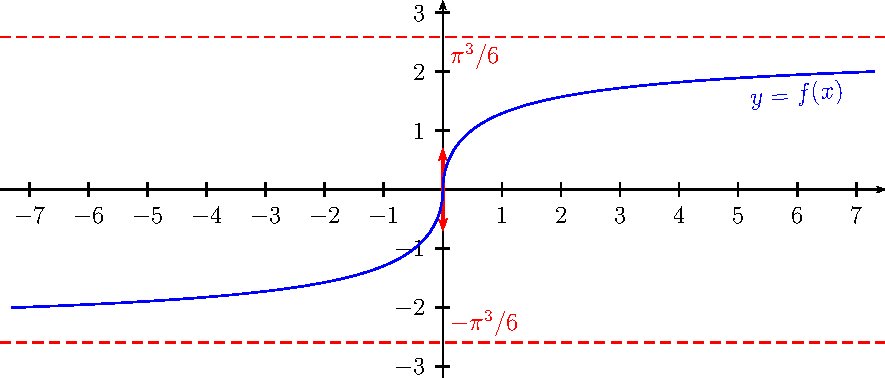
\includegraphics{../images/pdf/zjvO-1.pdf}$$
}
}
